% Copyright 2004 by Till Tantau <tantau@users.sourceforge.net>.
%
% In principle, this file can be redistributed and/or modified under
% the terms of the GNU Public License, version 2.
%
% However, this file is supposed to be a template to be modified
% for your own needs. For this reason, if you use this file as a
% template and not specifically distribute it as part of a another
% package/program, I grant the extra permission to freely copy and
% modify this file as you see fit and even to delete this copyright
% notice. 

\documentclass{beamer}

% There are many different themes available for Beamer. A comprehensive
% list with examples is given here:
% http://deic.uab.es/~iblanes/beamer_gallery/index_by_theme.html
% You can uncomment the themes below if you would like to use a different
% one:
%\usetheme{AnnArbor}
%\usetheme{Antibes}
%\usetheme{Bergen}
%\usetheme{Berkeley}
%\usetheme{Berlin}
%\usetheme{Boadilla}
%\usetheme{boxes}
%\usetheme{CambridgeUS}
%\usetheme{Copenhagen}
%\usetheme{Darmstadt}
%\usetheme{default}
%\usetheme{Frankfurt}
%\usetheme{Goettingen}
%\usetheme{Hannover}
%\usetheme{Ilmenau}
%\usetheme{JuanLesPins}
%\usetheme{Luebeck}
%\usetheme{Madrid}
%\usetheme{Malmoe}
%\usetheme{Marburg}
%\usetheme{Montpellier}
%\usetheme{PaloAlto}
%\usetheme{Pittsburgh}
%\usetheme{Rochester}
%\usetheme{Singapore}
%\usetheme{Szeged}
\usetheme{Warsaw}

\usepackage[brazil]{babel}
\usepackage[utf8]{inputenc}

% Add page to template
\addtobeamertemplate{navigation symbols}{}{%
    \usebeamerfont{footline}%
    \usebeamercolor[fg]{footline}%
    \hspace{1em}%
    \insertframenumber/\inserttotalframenumber
}

\title[Colab - Um framework de Integração de Aplicações Web]
{Colab - Um framework de Integração de\\Aplicações Web: Desenvolvimento e Aplicação}

% A subtitle is optional and this may be deleted
\subtitle{Exame de Qualificação}

\author[Sérgio Oliveira Campos (ICMC) – 2016]{Sérgio Oliveira Campos\inst{1}\\{\small Orientador: Prof. José Carlos Maldonado\inst{1}}\\{\small Orientador: Prof. Paulo Meirelles\inst{2}}}
% - Give the names in the same order as the appear in the paper.
% - Use the \inst{?} command only if the authors have different
%   affiliation.

\institute[ICMC] % (optional)
{
  \inst{1}%
  Instituto de Ciências Matemáticas e de Computação – ICMC\\
  Universidade de São Paulo
  
  \and
  \inst{2}%
  Faculdade de Engenharias do Gama – FGA\\
  Universidade de Brasília
}
% - Use the \inst command only if there are several affiliations.
% - Keep it simple, no one is interested in your street address.

\date{Maio 2016}
% - Either use conference name or its abbreviation.
% - Not really informative to the audience, more for people (including
%   yourself) who are reading the slides online

\logo{
\includegraphics[height=0.7cm]{logo_icmc.png}}

%\subject{Theoretical Computer Science}
% This is only inserted into the PDF information catalog. Can be left
% out. 

% If you have a file called "university-logo-filename.xxx", where xxx
% is a graphic format that can be processed by latex or pdflatex,
% resp., then you can add a logo as follows:

\pgfdeclareimage[height=0.5cm]{university-logo}{logo_icmc.png}
\logo{\pgfuseimage{university-logo}}

% Delete this, if you do not want the table of contents to pop up at
% the beginning of each subsection:
%\AtBeginSubsection[]
%{
%  \begin{frame}<beamer>{Outline}
%    \tableofcontents[currentsection,currentsubsection]
%  \end{frame}
%}

% Let's get started
\begin{document}

\begin{frame}
  \titlepage
\end{frame}

\begin{frame}{Sumário}
  \tableofcontents
  % You might wish to add the option [pausesections]
\end{frame}

% Section and subsections will appear in the presentation overview
% and table of contents.
\section{Introdução}

\subsection{Contexto}

\begin{frame}{Contextualização}

  \begin{itemize}
  \item {
    A Web como plataforma \cite{OReilly2007}
  }
  \item{
    Computação em nuvem
  }
  \item {
    Crescente uso de aplicações Web
  }
  \end{itemize}
 
\end{frame}


\begin{frame}{Problema}

  Dificuldade para os usuários:  
  \begin{itemize}
  \item {
    Aprender a utilizar múltiplas ferramentas
  }
  \item {
    Recordar múltiplas credenciais de acesso
  }
  \item {
    Ações redundantes entre ferramentas
  }
  \end{itemize}
\end{frame}

\begin{frame}{Problema}
  Dificuldades para as organizações:
  \begin{itemize}

  \item {
    Trabalhar com conjuntos de dados redundantes
  }
  \item {
    Garantir a segurança de múltiplos sistemas
  }
  \item {
    Visualizar e cruzar informações vindas de sistemas distintos
  }
  \item {
    Evitar inconsistência
  }
  
  \end{itemize}
\end{frame}

\subsection{Trabalhos Relacionados}

% You can reveal the parts of a slide one at a time
% with the \pause command:
\begin{frame}{Trabalhos Relacionados}
  \begin{itemize}
  \item {
    First item.
    \pause % The slide will pause after showing the first item
  }
  \item {   
    Second item.
  }
  % You can also specify when the content should appear
  % by using <n->:
  \item<3-> {
    Third item.
  }
  \item<4-> {
    Fourth item.
  }
  % or you can use the \uncover command to reveal general
  % content (not just \items):
  \item<5-> {
    Fifth item. \uncover<6->{Extra text in the fifth item.}
  }
  \end{itemize}
\end{frame}

\subsection{Terminologia e Conceitos}

\begin{frame}{Conceitos}
    \begin{block}{Famílias de web sites}
     \textit{``Web Site Families organize related web sites in a hierarchy in which common design requirements for members at a lower level (e.g., department web site) are defined at the higher level (e.g., faculty level).''} \cite{Eichinger2009}
    \end{block}
    \begin{theorem}
    There are separate environments for theorems, examples, definitions and proofs.
    \end{theorem}
    \begin{example}
    Here is an example of an example block.
    \end{example}
\end{frame}

\section{Integrações}

\begin{frame}{Colab}
  \begin{itemize}
  \item {
    My first point.
  }
  \item {
    My second point.
  }
  \end{itemize}
\end{frame}

\subsection{Autenticação}

\begin{frame}{Integração de Autenticação}
  \begin{itemize}
  \item {
    My first point.
  }
  \item {
    My second point.
  }
  \end{itemize}
\end{frame}

\subsection{Visual}

\begin{frame}{Integração Visual}
  \begin{itemize}
  \item {
    My first point.
  }
  \item {
    My second point.
  }
  \end{itemize}
\end{frame}

\subsection{Eventos}

\begin{frame}{Integração por Eventos}
  \begin{itemize}
  \item {
    My first point.
  }
  \item {
    My second point.
  }
  \end{itemize}
\end{frame}

\subsection{Dados e Busca}

\begin{frame}{Integração de Dados e Busca}
  \begin{itemize}
  \item {
    My first point.
  }
  \item {
    My second point.
  }
  \end{itemize}
\end{frame}

\section{Limitações}

\begin{frame}{Limitações do Trabalho}
  \begin{itemize}
  \item {
    My first point.
  }
  \item {
    My second point.
  }
  \end{itemize}
\end{frame}

\section{Plano de trabalho}

\begin{frame}{Plano de Trabalho}
    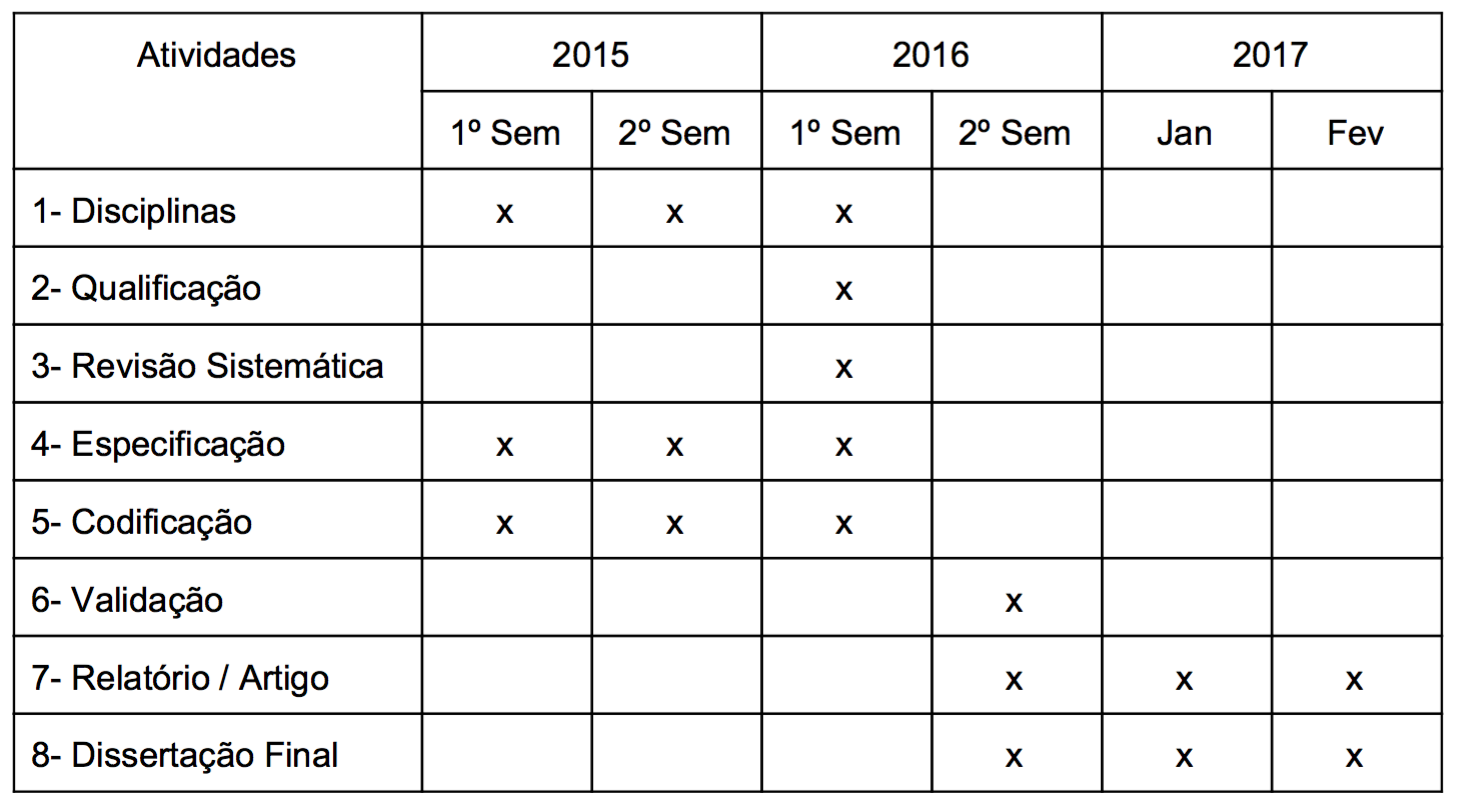
\includegraphics[scale=0.4]{plano_de_trabalho}
\end{frame}

% All of the following is optional and typically not needed. 
\section*{Referências}

\begin{frame}[allowframebreaks]
    \frametitle{Referências}
    \bibliographystyle{apalike}
    \bibliography{references.bib}
\end{frame}

\end{document}